\documentclass[11pt]{article}
\usepackage[notes]{la}
\lamodule{4}{6}{Change of Basis}
\laxdoc{4.4}
\laxdoc{4.5}

\begin{document}

\section{Change of Basis}

\begin{guide}
In Section 4.4 the vector $\bv{x}=(4,5)$ had the coordinate vector $(3,2)$ in the basis $\mathcal{B}=\{(2,1),(-1,1)\}$ and the coordinate vector $(\tfrac92,-\tfrac12)$ in the basis $\mathcal{D}=\{(1,1),(1,-1)\}$ (Example~\ref{4.4-ex:samenums}). The vector did not change; only the coordinate system did. Is there a rule that turns the first list of numbers into the second without going back to the vector itself? Is the rule linear, so that a single matrix does it for every vector at once? And since the same rule must be able to run backwards, what kind of matrix can it be?
\end{guide}

\textbf{This section is an enrichment.} It is a good place to see the coordinate mapping of Section 4.4 and the dimension count of Section 4.5 work together.

\textbf{By the end of this section you should be able to:}
\begin{itemize}
  \item state what the change-of-basis matrix $P_{\mathcal{C}\leftarrow\mathcal{B}}$ does, say why it is square, and explain why its columns are the $\mathcal{C}$-coordinates of the vectors of $\mathcal{B}$;
  \item write down $P_{\mathcal{C}\leftarrow\mathcal{B}}$ directly when each $\bv{b}_j$ is given as a combination of the $\bv{c}_i$, and use it to convert coordinates in both directions;
  \item compute $P_{\mathcal{C}\leftarrow\mathcal{B}}$ by row reducing $[\,\mathcal{C}\mid\mathcal{B}\,]$ to $[\,I\mid P_{\mathcal{C}\leftarrow\mathcal{B}}\,]$ in $\R^2$, in $\R^3$, in $\mathbb{P}_n$, in $M_{2\times2}$, in a plane inside $\R^3$ and in a space of functions;
  \item explain why $P_{\mathcal{B}\leftarrow\mathcal{C}}=\left(P_{\mathcal{C}\leftarrow\mathcal{B}}\right)^{-1}$ and why every change-of-basis matrix is invertible;
  \item change coordinates in two steps, through the standard basis, and use $P_{\mathcal{D}\leftarrow\mathcal{B}}=P_{\mathcal{D}\leftarrow\mathcal{C}}\,P_{\mathcal{C}\leftarrow\mathcal{B}}$;
  \item decide whether a given matrix can be a change-of-basis matrix, and recover a basis $\mathcal{B}$ from $\mathcal{C}$ and $P_{\mathcal{C}\leftarrow\mathcal{B}}$.
\end{itemize}

% ---------------------------------------------------------------------
\subsection*{One vector, two coordinate vectors}

Let $\mathcal{B}$ and $\mathcal{C}$ be two bases of the same vector space $V$. A vector $\bv{x}$ in $V$ has a coordinate vector $[\bv{x}]_{\mathcal{B}}$ and a coordinate vector $[\bv{x}]_{\mathcal{C}}$. The first determines the vector (Theorem~\ref{4.4-thm:unique}), and the vector determines the second, so $[\bv{x}]_{\mathcal{B}}$ determines $[\bv{x}]_{\mathcal{C}}$. The new fact is that the passage from one to the other is multiplication by a matrix. The reason is the linearity of the coordinate mapping (Theorem~\ref{4.4-thm:coordmap}): the map that sends $[\bv{x}]_{\mathcal{B}}$ first to $\bv{x}$ and then to $[\bv{x}]_{\mathcal{C}}$ is a composition of two linear maps. The theorem also tells us what the matrix is.

\begin{thm}{The change-of-basis matrix}{matrix}
Let $\mathcal{B}=\{\bv{b}_1,\dots,\bv{b}_n\}$ and $\mathcal{C}=\{\bv{c}_1,\dots,\bv{c}_m\}$ be bases for the same vector space $V$. Then $m=n$, and there is exactly one $n\times n$ matrix $P_{\mathcal{C}\leftarrow\mathcal{B}}$ such that
\[
[\bv{x}]_{\mathcal{C}}=P_{\mathcal{C}\leftarrow\mathcal{B}}\,[\bv{x}]_{\mathcal{B}}\qquad\text{for every }\bv{x}\text{ in }V.
\]
Its columns are the $\mathcal{C}$-coordinate vectors of the vectors of $\mathcal{B}$:
\[
P_{\mathcal{C}\leftarrow\mathcal{B}}=\begin{bmatrix}[\bv{b}_1]_{\mathcal{C}}&[\bv{b}_2]_{\mathcal{C}}&\cdots&[\bv{b}_n]_{\mathcal{C}}\end{bmatrix}.
\]
\end{thm}

\begin{proof}
Both bases have the same number of vectors by Theorem~\ref{4.5-thm:samesize}, so $m=n$. Let $\bv{x}$ be in $V$ and write $\bv{x}=r_1\bv{b}_1+\cdots+r_n\bv{b}_n$, so that $[\bv{x}]_{\mathcal{B}}=(r_1,\dots,r_n)$. The coordinate mapping of $\mathcal{C}$ is linear (Theorem~\ref{4.4-thm:coordmap}), hence
\[
[\bv{x}]_{\mathcal{C}}=r_1[\bv{b}_1]_{\mathcal{C}}+\cdots+r_n[\bv{b}_n]_{\mathcal{C}}=\begin{bmatrix}[\bv{b}_1]_{\mathcal{C}}&\cdots&[\bv{b}_n]_{\mathcal{C}}\end{bmatrix}\begin{bmatrix}r_1\\\vdots\\r_n\end{bmatrix},
\]
which is the matrix $P_{\mathcal{C}\leftarrow\mathcal{B}}$ of the statement times $[\bv{x}]_{\mathcal{B}}$. For uniqueness, suppose $M$ is an $n\times n$ matrix with $[\bv{x}]_{\mathcal{C}}=M[\bv{x}]_{\mathcal{B}}$ for all $\bv{x}$. Take $\bv{x}=\bv{b}_j$. Then $[\bv{b}_j]_{\mathcal{B}}=\bv{e}_j$ (Example~\ref{4.4-ex:bj}), so $M\bv{e}_j$, the $j$th column of $M$, equals $[\bv{b}_j]_{\mathcal{C}}$. The columns of $M$ are the columns of $P_{\mathcal{C}\leftarrow\mathcal{B}}$.
\end{proof}

\begin{think}{Why square?}{square}
(a)~In the proof, where did the number of rows and the number of columns of the matrix come from, and which earlier theorem makes them equal? (b)~If $V$ has dimension $5$, what is the size of $P_{\mathcal{C}\leftarrow\mathcal{B}}$ for two bases $\mathcal{B}$ and $\mathcal{C}$ of $V$? (c)~A student claims that a $3\times2$ matrix converts coordinates relative to a basis with $2$ vectors into coordinates relative to a basis with $3$ vectors of the same space. Why is there no such pair of bases?
\end{think}

\begin{defn}{Change-of-basis matrix}{PCB}
The matrix $P_{\mathcal{C}\leftarrow\mathcal{B}}$ of Theorem~\ref{thm:matrix} is the \emph{change-of-basis matrix from $\mathcal{B}$ to $\mathcal{C}$}. The arrow shows the way the coordinates travel, and the symbol is read from right to left, as a product acts: $[\bv{x}]_{\mathcal{B}}$ goes in on the right and $[\bv{x}]_{\mathcal{C}}$ comes out on the left.
\end{defn}

\begin{warn}[Direction matters]
The $j$th column of $P_{\mathcal{C}\leftarrow\mathcal{B}}$ is $[\bv{b}_j]_{\mathcal{C}}$: the $\mathcal{C}$-coordinates of the $\mathcal{B}$-vectors, not the $\mathcal{B}$-coordinates of the $\mathcal{C}$-vectors. The matrix $P_{\mathcal{B}\leftarrow\mathcal{C}}$ is a different matrix in general. When you have computed a column, ask which basis it is a combination of: the numbers in the column are the weights on the vectors of the \emph{target} basis $\mathcal{C}$.
\end{warn}

\begin{exmp}{The two coordinate vectors of $(4,5)$}{D2}
Let $\mathcal{B}=\{\bv{b}_1,\bv{b}_2\}=\{(2,1),(-1,1)\}$ and $\mathcal{D}=\{\bv{d}_1,\bv{d}_2\}=\{(1,1),(1,-1)\}$ be the bases of $\R^2$ of Example~\ref{4.4-ex:samenums}. We find $P_{\mathcal{D}\leftarrow\mathcal{B}}$, whose columns are $[\bv{b}_1]_{\mathcal{D}}$ and $[\bv{b}_2]_{\mathcal{D}}$. Each is the solution of a system whose coefficient columns are $\bv{d}_1,\bv{d}_2$: $\bv{d}_1c_1+\bv{d}_2c_2=\bv{b}_1$ and $\bv{d}_1c_1+\bv{d}_2c_2=\bv{b}_2$. Both systems have the same coefficient matrix, so we solve them together by row reducing the matrix $[\,\bv{d}_1\ \bv{d}_2\mid\bv{b}_1\ \bv{b}_2\,]$:
\begin{align*}
\begin{amat}{cc|cc}1 & 1 & 2 & -1\\1 & -1 & 1 & 1\end{amat}
&\rops{R_2-R_1}
\begin{amat}{cc|cc}1 & 1 & 2 & -1\\0 & -2 & -1 & 2\end{amat}
\rops{-\tfrac{1}{2}R_2}
\begin{amat}{cc|cc}1 & 1 & 2 & -1\\0 & 1 & \tfrac{1}{2} & -1\end{amat}
\\[4pt]
&\rops{R_1-R_2}
\begin{amat}{cc|cc}1 & 0 & \tfrac{3}{2} & 0\\0 & 1 & \tfrac{1}{2} & -1\end{amat}
\end{align*}
The right half is $P_{\mathcal{D}\leftarrow\mathcal{B}}$:
\[
P_{\mathcal{D}\leftarrow\mathcal{B}}=\begin{bmatrix}\tfrac32&0\\\tfrac12&-1\end{bmatrix},\qquad\text{that is}\qquad \bv{b}_1=\tfrac32\bv{d}_1+\tfrac12\bv{d}_2,\quad \bv{b}_2=0\,\bv{d}_1-\bv{d}_2.
\]
Check the columns: $\tfrac32(1,1)+\tfrac12(1,-1)=(2,1)$ and $-(1,-1)=(-1,1)$. \ $\checkmark$ Now use the matrix on the vector $\bv{x}=(4,5)$, whose $\mathcal{B}$-coordinates are $(3,2)$:
\[
[\bv{x}]_{\mathcal{D}}=\begin{bmatrix}\tfrac32&0\\\tfrac12&-1\end{bmatrix}\begin{bmatrix}3\\2\end{bmatrix}=\begin{bmatrix}\tfrac92\\-\tfrac12\end{bmatrix}.
\]
This is the coordinate vector $(\tfrac92,-\tfrac12)$ that Example~\ref{4.4-ex:samenums} found by going through $\bv{x}$ itself. The matrix gets there without ever writing down $\bv{x}$.
\end{exmp}

\begin{center}
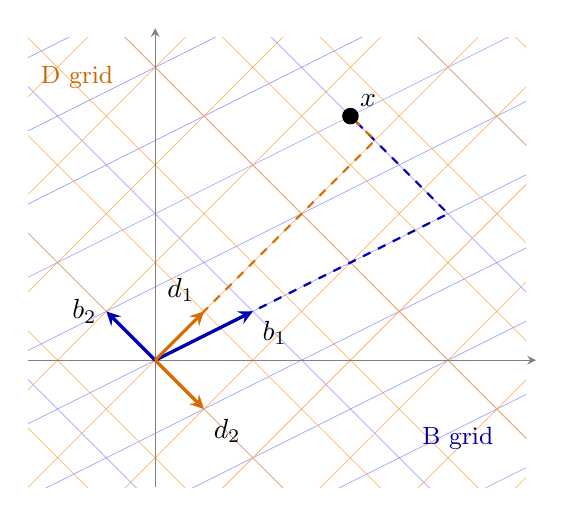
\begin{tikzpicture}[x=0.62cm,y=0.62cm,>=stealth]
  \begin{scope}
    \clip (-2.6,-2.6) rectangle (7.6,6.6);
    \begin{scope}[cm={2,1,-1,1,(0,0)}]
      \draw[blue!45,very thin] (-8,-8) grid[step=1] (8,8);
    \end{scope}
    \begin{scope}[cm={1,1,1,-1,(0,0)}]
      \draw[orange!70,very thin] (-8,-8) grid[step=1] (8,8);
    \end{scope}
  \end{scope}
  \draw[->,gray] (-2.6,0)--(7.8,0);
  \draw[->,gray] (0,-2.6)--(0,6.8);
  \draw[dashed,thick,blue!70!black] (0,0)--(6,3)--(4,5);
  \draw[dashed,thick,orange!85!black] (0,0)--(4.5,4.5)--(4,5);
  \draw[->,very thick,blue!70!black] (0,0)--(2,1);
  \draw[->,very thick,blue!70!black] (0,0)--(-1,1);
  \draw[->,very thick,orange!85!black] (0,0)--(1,1);
  \draw[->,very thick,orange!85!black] (0,0)--(1,-1);
  \fill (4,5) circle (3pt);
  \node[below right] at (2,1) {$b_1$};
  \node[left] at (-1,1) {$b_2$};
  \node[above left] at (1,1) {$d_1$};
  \node[below right] at (1,-1) {$d_2$};
  \node[above right] at (4,5) {$x$};
  \node[blue!60!black] at (6.2,-1.6) {\small B grid};
  \node[orange!80!black] at (-1.6,5.8) {\small D grid};
\end{tikzpicture}
\end{center}

\textbf{Figure 1.} Two coordinate grids on the same plane. The blue grid is drawn with the axes $\bv{b}_1=(2,1)$ and $\bv{b}_2=(-1,1)$ and the orange grid with the axes $\bv{d}_1=(1,1)$ and $\bv{d}_2=(1,-1)$. The point $\bv{x}=(4,5)$ is reached by three steps along $\bv{b}_1$ and two along $\bv{b}_2$ (blue dashed path), so $[\bv{x}]_{\mathcal{B}}=(3,2)$; it is also reached by four and a half steps along $\bv{d}_1$ and one half step \emph{backwards} along $\bv{d}_2$ (orange dashed path), so $[\bv{x}]_{\mathcal{D}}=(\tfrac92,-\tfrac12)$. The point is the same. The matrix $P_{\mathcal{D}\leftarrow\mathcal{B}}$ converts the first pair of numbers into the second.

\begin{think}{Reading the two grids}{grids}
(a)~In Figure~1, what are the coordinates of the corner reached by the blue path, as a corner of the orange grid? (b)~Which column of $P_{\mathcal{D}\leftarrow\mathcal{B}}$ tells you how to reach the tip of the blue arrow $\bv{b}_1$ by orange steps, and what are the steps? (c)~Of the plane, the point $\bv{x}$ and its coordinates, which changed when we passed from the blue grid to the orange grid?
\end{think}

\subsection*{The inverse of a change-of-basis matrix}

Nothing in Theorem~\ref{thm:matrix} favours $\mathcal{B}$ over $\mathcal{C}$. Exchanging the roles gives a second matrix, $P_{\mathcal{B}\leftarrow\mathcal{C}}$, with $[\bv{x}]_{\mathcal{B}}=P_{\mathcal{B}\leftarrow\mathcal{C}}[\bv{x}]_{\mathcal{C}}$. Going from $\mathcal{B}$ to $\mathcal{C}$ and then back to $\mathcal{B}$ must return the coordinates we started with.

\begin{thm}{The inverse of a change-of-basis matrix}{inverse}
Let $\mathcal{B}$ and $\mathcal{C}$ be bases of an $n$-dimensional vector space $V$.
\begin{enumerate}[label=(\alph*),itemsep=1pt]
  \item $P_{\mathcal{B}\leftarrow\mathcal{B}}=I$.
  \item $P_{\mathcal{B}\leftarrow\mathcal{C}}\,P_{\mathcal{C}\leftarrow\mathcal{B}}=I$ and $P_{\mathcal{C}\leftarrow\mathcal{B}}\,P_{\mathcal{B}\leftarrow\mathcal{C}}=I$. Hence $P_{\mathcal{C}\leftarrow\mathcal{B}}$ is invertible and $\left(P_{\mathcal{C}\leftarrow\mathcal{B}}\right)^{-1}=P_{\mathcal{B}\leftarrow\mathcal{C}}$.
\end{enumerate}
\end{thm}

\begin{proof}
(a)~$[\bv{x}]_{\mathcal{B}}=I[\bv{x}]_{\mathcal{B}}$ for every $\bv{x}$, and the matrix in Theorem~\ref{thm:matrix} is unique. (b)~For every $\bv{x}$ in $V$,
\[
[\bv{x}]_{\mathcal{B}}=P_{\mathcal{B}\leftarrow\mathcal{C}}[\bv{x}]_{\mathcal{C}}=P_{\mathcal{B}\leftarrow\mathcal{C}}P_{\mathcal{C}\leftarrow\mathcal{B}}[\bv{x}]_{\mathcal{B}}.
\]
The coordinate mapping of $\mathcal{B}$ is onto $\R^n$ (Theorem~\ref{4.4-thm:coordmap}), so every $\bv{y}$ in $\R^n$ has the form $[\bv{x}]_{\mathcal{B}}$, and the equation says $\bv{y}=P_{\mathcal{B}\leftarrow\mathcal{C}}P_{\mathcal{C}\leftarrow\mathcal{B}}\bv{y}$ for every $\bv{y}$. Taking $\bv{y}=\bv{e}_1,\dots,\bv{e}_n$ shows that the product is the identity matrix. The other product is the same argument with $\mathcal{B}$ and $\mathcal{C}$ exchanged.
\end{proof}

\begin{think}{Zero columns and zero rows}{rows}
(a)~Why can a change-of-basis matrix never have a column of zeros? (Which vector would that column describe?) (b)~Why can it never have a row of zeros? (Think of the basis vector $\bv{c}_i$ and its $\mathcal{C}$-coordinate vector.) (c)~Theorem~\ref{thm:inverse} gives invertibility. Which of the two observations in (a) and (b) is a first symptom of it?
\end{think}

\begin{exmp}{Abstract bases: reading the matrix from the formulas}{abstract}
Let $\mathcal{B}=\{\bv{b}_1,\bv{b}_2\}$ and $\mathcal{C}=\{\bv{c}_1,\bv{c}_2\}$ be bases of a vector space $V$ with
\[
\bv{b}_1=2\bv{c}_1-\bv{c}_2,\qquad \bv{b}_2=-3\bv{c}_1+2\bv{c}_2.
\]
No vectors are given as lists of numbers, and none are needed. The formulas say $[\bv{b}_1]_{\mathcal{C}}=(2,-1)$ and $[\bv{b}_2]_{\mathcal{C}}=(-3,2)$, so
\[
P_{\mathcal{C}\leftarrow\mathcal{B}}=\begin{bmatrix}2&-3\\-1&2\end{bmatrix}.
\]
Its determinant is $4-3=1$, and the formula for the inverse of a $2\times2$ matrix (Section 2.2) gives
\[
P_{\mathcal{B}\leftarrow\mathcal{C}}=\left(P_{\mathcal{C}\leftarrow\mathcal{B}}\right)^{-1}=\begin{bmatrix}2&3\\1&2\end{bmatrix},\qquad \begin{bmatrix}2&-3\\-1&2\end{bmatrix}\begin{bmatrix}2&3\\1&2\end{bmatrix}=\begin{bmatrix}1&0\\0&1\end{bmatrix}.
\]
The columns of the inverse express the $\bv{c}_i$ in terms of the $\bv{b}_j$: $\bv{c}_1=2\bv{b}_1+\bv{b}_2$ and $\bv{c}_2=3\bv{b}_1+2\bv{b}_2$. Check: $2\bv{b}_1+\bv{b}_2=4\bv{c}_1-2\bv{c}_2-3\bv{c}_1+2\bv{c}_2=\bv{c}_1$. \ $\checkmark$

Now convert coordinates in both directions. If $[\bv{x}]_{\mathcal{B}}=(4,-1)$ then
\[
[\bv{x}]_{\mathcal{C}}=\begin{bmatrix}2&-3\\-1&2\end{bmatrix}\begin{bmatrix}4\\-1\end{bmatrix}=\begin{bmatrix}11\\-6\end{bmatrix},
\]
and if $[\bv{y}]_{\mathcal{C}}=(5,3)$ then
\[
[\bv{y}]_{\mathcal{B}}=\begin{bmatrix}2&3\\1&2\end{bmatrix}\begin{bmatrix}5\\3\end{bmatrix}=\begin{bmatrix}19\\11\end{bmatrix}.
\]
Check the first: $4\bv{b}_1-\bv{b}_2=4(2\bv{c}_1-\bv{c}_2)-(-3\bv{c}_1+2\bv{c}_2)=11\bv{c}_1-6\bv{c}_2$. \ $\checkmark$
\end{exmp}

\begin{think}{Easy changes: reordering, scaling and doing nothing}{special}
(a)~Let $\mathcal{C}=\{\bv{b}_2,\bv{b}_1\}$ be the basis $\mathcal{B}=\{\bv{b}_1,\bv{b}_2\}$ with its two vectors listed in the other order. Find $P_{\mathcal{C}\leftarrow\mathcal{B}}$. (b)~Let $\mathcal{C}=\{2\bv{b}_1,2\bv{b}_2\}$. Find $P_{\mathcal{C}\leftarrow\mathcal{B}}$. (c)~Show that $P_{\mathcal{C}\leftarrow\mathcal{B}}=I$ if and only if $\mathcal{C}=\mathcal{B}$ as lists, in the same order. Why does the order of a basis matter for the matrix?
\end{think}

\begin{kc}{Reading a matrix from the formulas}{cols}
Let $\mathcal{B}=\{\bv{b}_1,\bv{b}_2,\bv{b}_3\}$ and $\mathcal{C}=\{\bv{c}_1,\bv{c}_2,\bv{c}_3\}$ be bases of a vector space, with $\bv{b}_1=\bv{c}_1-\bv{c}_2$, $\bv{b}_2=\bv{c}_2+\bv{c}_3$ and $\bv{b}_3=2\bv{c}_1+\bv{c}_3$. (a)~Write $P_{\mathcal{C}\leftarrow\mathcal{B}}$. (b)~If $[\bv{x}]_{\mathcal{B}}=(1,2,-1)$, find $[\bv{x}]_{\mathcal{C}}$. (c)~Given that $P_{\mathcal{B}\leftarrow\mathcal{C}}=\begin{bmatrix}-1&-2&2\\-1&-1&2\\1&1&-1\end{bmatrix}$, write $\bv{c}_1$ as a combination of $\bv{b}_1,\bv{b}_2,\bv{b}_3$.
\end{kc}

% ---------------------------------------------------------------------
\subsection*{Computing the matrix in $\R^n$}

When the vectors of both bases are lists of numbers, we do not need to solve one system per column. The matrix $P_{\mathcal{B}}$ of Theorem~\ref{4.4-thm:PB} does all the work.

\begin{thm}{Change of basis in $\R^n$}{formula}
Let $\mathcal{B}=\{\bv{b}_1,\dots,\bv{b}_n\}$ and $\mathcal{C}=\{\bv{c}_1,\dots,\bv{c}_n\}$ be bases for $\R^n$, and put $P_{\mathcal{B}}=\begin{bmatrix}\bv{b}_1&\cdots&\bv{b}_n\end{bmatrix}$ and $P_{\mathcal{C}}=\begin{bmatrix}\bv{c}_1&\cdots&\bv{c}_n\end{bmatrix}$. Then
\[
P_{\mathcal{C}\leftarrow\mathcal{B}}=P_{\mathcal{C}}^{-1}P_{\mathcal{B}},
\]
and row reduction takes the matrix $[\,P_{\mathcal{C}}\mid P_{\mathcal{B}}\,]$ to $[\,I\mid P_{\mathcal{C}\leftarrow\mathcal{B}}\,]$.
\end{thm}

\begin{proof}
By Theorem~\ref{4.4-thm:PB}, $\bv{x}=P_{\mathcal{B}}[\bv{x}]_{\mathcal{B}}$ and $[\bv{x}]_{\mathcal{C}}=P_{\mathcal{C}}^{-1}\bv{x}$ for every $\bv{x}$ in $\R^n$. Therefore $[\bv{x}]_{\mathcal{C}}=P_{\mathcal{C}}^{-1}P_{\mathcal{B}}[\bv{x}]_{\mathcal{B}}$, and by the uniqueness in Theorem~\ref{thm:matrix} the matrix $P_{\mathcal{C}}^{-1}P_{\mathcal{B}}$ is $P_{\mathcal{C}\leftarrow\mathcal{B}}$. For the second statement, the row operations that reduce the invertible matrix $P_{\mathcal{C}}$ to $I$ are multiplication on the left by $P_{\mathcal{C}}^{-1}$ (this is the reasoning behind the inverse algorithm of Section 2.2); applied to the whole matrix $[\,P_{\mathcal{C}}\mid P_{\mathcal{B}}\,]$ they produce $[\,P_{\mathcal{C}}^{-1}P_{\mathcal{C}}\mid P_{\mathcal{C}}^{-1}P_{\mathcal{B}}\,]=[\,I\mid P_{\mathcal{C}\leftarrow\mathcal{B}}\,]$.
\end{proof}

The same idea works in every space with a basis whose coordinates we know. In $\mathbb{P}_n$ we write each polynomial by its coefficient vector, in $M_{2\times2}$ each matrix by its entries read row by row, and in a plane inside $\R^3$ the vectors are lists already. Section 4.4 showed that the coordinate mapping of a fixed basis $\mathcal{E}$ of that kind lets us do all the arithmetic in $\R^n$ (Theorem~\ref{4.4-thm:transfer} and Procedure~\ref{4.4-proc:testcoords}). The same computation gives the matrix.

\begin{proc}{Computing $P_{\mathcal{C}\leftarrow\mathcal{B}}$ by row reduction}{rowred}
Let $\mathcal{B}=\{\bv{b}_1,\dots,\bv{b}_n\}$ and $\mathcal{C}=\{\bv{c}_1,\dots,\bv{c}_n\}$ be bases of $V$, and let $\mathcal{E}$ be a basis in which coordinates are easy to write (the standard basis of $\R^n$, of $\mathbb{P}_n$ or of $M_{2\times2}$, say).
\begin{enumerate}[label=\arabic*.,itemsep=1pt]
  \item Write the $\mathcal{E}$-coordinate columns of the vectors of $\mathcal{C}$ on the left and those of $\mathcal{B}$ on the right: $[\,[\bv{c}_1]_{\mathcal{E}}\cdots[\bv{c}_n]_{\mathcal{E}}\mid[\bv{b}_1]_{\mathcal{E}}\cdots[\bv{b}_n]_{\mathcal{E}}\,]$.
  \item Row reduce. The left half becomes $I$ (it must, since $\mathcal{C}$ is a basis) and the right half becomes $P_{\mathcal{C}\leftarrow\mathcal{B}}$.
  \item Check one column: $\bv{b}_j$ should equal the combination of the $\bv{c}_i$ with the weights in column $j$.
\end{enumerate}
To get $P_{\mathcal{B}\leftarrow\mathcal{C}}$ instead, either invert the matrix you have (Theorem~\ref{thm:inverse}) or reduce $[\,\mathcal{B}\mid\mathcal{C}\,]$.
\end{proc}

\begin{think}{Which side goes on the left?}{direction}
(a)~Row reducing $[\,\mathcal{C}\mid\mathcal{B}\,]$ gives $P_{\mathcal{C}\leftarrow\mathcal{B}}$. What does row reducing $[\,\mathcal{B}\mid\mathcal{C}\,]$ give, and why? (b)~Suppose you row reduce $[\,\mathcal{C}\mid\mathcal{B}\,]$ and the left half does not reach $I$. What does that tell you about the set $\mathcal{C}$? (c)~You already know $P_{\mathcal{C}\leftarrow\mathcal{B}}$ and want $P_{\mathcal{B}\leftarrow\mathcal{C}}$. Name two ways to get it and say when each is quicker.
\end{think}

\begin{exmp}{Two arbitrary bases of $\R^2$}{R2a}
Let $\mathcal{B}=\{(1,-2),(3,-5)\}$ and $\mathcal{C}=\{(2,1),(5,3)\}$. Row reduce $[\,\bv{c}_1\ \bv{c}_2\mid\bv{b}_1\ \bv{b}_2\,]$:
\begin{align*}
\begin{amat}{cc|cc}2 & 5 & 1 & 3\\1 & 3 & -2 & -5\end{amat}
&\rops{R_1\leftrightarrow R_2}
\begin{amat}{cc|cc}1 & 3 & -2 & -5\\2 & 5 & 1 & 3\end{amat}
\rops{R_2-2R_1}
\begin{amat}{cc|cc}1 & 3 & -2 & -5\\0 & -1 & 5 & 13\end{amat}
\\[4pt]
&\rops{-R_2}
\begin{amat}{cc|cc}1 & 3 & -2 & -5\\0 & 1 & -5 & -13\end{amat}
\rops{R_1-3R_2}
\begin{amat}{cc|cc}1 & 0 & 13 & 34\\0 & 1 & -5 & -13\end{amat}
\end{align*}
Therefore
\[
P_{\mathcal{C}\leftarrow\mathcal{B}}=\begin{bmatrix}13&34\\-5&-13\end{bmatrix}.
\]
Check the first column: $13(2,1)-5(5,3)=(26-25,\ 13-15)=(1,-2)=\bv{b}_1$. \ $\checkmark$ The determinant is $-169+170=1$, so
\[
P_{\mathcal{B}\leftarrow\mathcal{C}}=\begin{bmatrix}13&34\\-5&-13\end{bmatrix}^{-1}=\begin{bmatrix}-13&-34\\5&13\end{bmatrix},\qquad \begin{bmatrix}13&34\\-5&-13\end{bmatrix}\begin{bmatrix}-13&-34\\5&13\end{bmatrix}=\begin{bmatrix}1&0\\0&1\end{bmatrix}.
\]
Finally, if $[\bv{x}]_{\mathcal{B}}=(2,-1)$, then $\bv{x}=2(1,-2)-(3,-5)=(-1,1)$ and
\[
[\bv{x}]_{\mathcal{C}}=\begin{bmatrix}13&34\\-5&-13\end{bmatrix}\begin{bmatrix}2\\-1\end{bmatrix}=\begin{bmatrix}-8\\3\end{bmatrix}.
\]
Check: $-8(2,1)+3(5,3)=(-16+15,\ -8+9)=(-1,1)=\bv{x}$. \ $\checkmark$
\end{exmp}

\begin{kc}{A change of basis in $\R^2$ with fractions}{R2}
Let $\mathcal{B}=\{(3,1),(1,2)\}$ and $\mathcal{C}=\{(2,1),(-1,1)\}$. (a)~Row reduce $[\,\mathcal{C}\mid\mathcal{B}\,]$ to find $P_{\mathcal{C}\leftarrow\mathcal{B}}$. (b)~Find $[\bv{x}]_{\mathcal{C}}$ if $[\bv{x}]_{\mathcal{B}}=(2,-1)$, and check it by computing $\bv{x}$ both ways. (c)~Find $P_{\mathcal{B}\leftarrow\mathcal{C}}$.
\end{kc}

\begin{exmp}{Two arbitrary bases of $\R^3$}{R3}
Let $\mathcal{B}=\{(1,0,1),(1,1,0),(0,1,1)\}$ and $\mathcal{C}=\{(1,1,1),(0,1,1),(0,0,1)\}$. Both are bases of $\R^3$: the matrix of $\mathcal{C}$ is triangular with $1$ on the diagonal, and $\det P_{\mathcal{B}}=2$. Row reduce $[\,\mathcal{C}\mid\mathcal{B}\,]$:
\begin{align*}
\begin{amat}{ccc|ccc}1 & 0 & 0 & 1 & 1 & 0\\1 & 1 & 0 & 0 & 1 & 1\\1 & 1 & 1 & 1 & 0 & 1\end{amat}
&\rops{R_2-R_1,\ R_3-R_1}
\begin{amat}{ccc|ccc}1 & 0 & 0 & 1 & 1 & 0\\0 & 1 & 0 & -1 & 0 & 1\\0 & 1 & 1 & 0 & -1 & 1\end{amat}
\\[4pt]
&\rops{R_3-R_2}
\begin{amat}{ccc|ccc}1 & 0 & 0 & 1 & 1 & 0\\0 & 1 & 0 & -1 & 0 & 1\\0 & 0 & 1 & 1 & -1 & 0\end{amat}
\end{align*}
So
\[
P_{\mathcal{C}\leftarrow\mathcal{B}}=\begin{bmatrix}1&1&0\\-1&0&1\\1&-1&0\end{bmatrix}.
\]
Check the third column: $0(1,1,1)+1(0,1,1)+0(0,0,1)=(0,1,1)=\bv{b}_3$. \ $\checkmark$ The reverse matrix has halves in it:
\[
P_{\mathcal{B}\leftarrow\mathcal{C}}=\begin{bmatrix}\tfrac12&0&\tfrac12\\\tfrac12&0&-\tfrac12\\\tfrac12&1&\tfrac12\end{bmatrix},\qquad \begin{bmatrix}\tfrac12&0&\tfrac12\\\tfrac12&0&-\tfrac12\\\tfrac12&1&\tfrac12\end{bmatrix}\begin{bmatrix}1&1&0\\-1&0&1\\1&-1&0\end{bmatrix}=\begin{bmatrix}1&0&0\\0&1&0\\0&0&1\end{bmatrix}.
\]
The product shows that the two matrices are inverses of each other. Column by column, the second matrix says $\bv{c}_1=\tfrac12\bv{b}_1+\tfrac12\bv{b}_2+\tfrac12\bv{b}_3$: indeed $\tfrac12\left((1,0,1)+(1,1,0)+(0,1,1)\right)=(1,1,1)$. \ $\checkmark$
\end{exmp}

\begin{exmp}{From a basis to the standard basis, and back}{tostd}
Let $\mathcal{E}=\{\bv{e}_1,\bv{e}_2,\bv{e}_3\}$ be the standard basis of $\R^3$ and $\mathcal{B}=\{(1,0,1),(1,1,1),(0,1,1)\}$. Since $[\bv{b}]_{\mathcal{E}}=\bv{b}$ for every $\bv{b}$ in $\R^3$, the columns of $P_{\mathcal{E}\leftarrow\mathcal{B}}$ are the vectors $\bv{b}_j$ themselves:
\[
P_{\mathcal{E}\leftarrow\mathcal{B}}=P_{\mathcal{B}}=\begin{bmatrix}1&1&0\\0&1&1\\1&1&1\end{bmatrix}.
\]
No computation is needed: Theorem~\ref{4.4-thm:PB} is the special case $\mathcal{C}=\mathcal{E}$ of this section. The computation goes the other way. To get $P_{\mathcal{B}\leftarrow\mathcal{E}}=P_{\mathcal{B}}^{-1}$ (the matrix that produces $\mathcal{B}$-coordinates from the ordinary coordinates) reduce $[\,P_{\mathcal{B}}\mid I\,]$:
\begin{align*}
\begin{amat}{ccc|ccc}1 & 1 & 0 & 1 & 0 & 0\\0 & 1 & 1 & 0 & 1 & 0\\1 & 1 & 1 & 0 & 0 & 1\end{amat}
&\rops{R_3-R_1}
\begin{amat}{ccc|ccc}1 & 1 & 0 & 1 & 0 & 0\\0 & 1 & 1 & 0 & 1 & 0\\0 & 0 & 1 & -1 & 0 & 1\end{amat}
\\[4pt]
&\rops{R_1-R_2}
\begin{amat}{ccc|ccc}1 & 0 & -1 & 1 & -1 & 0\\0 & 1 & 1 & 0 & 1 & 0\\0 & 0 & 1 & -1 & 0 & 1\end{amat}
\\[4pt]
&\rops{R_1+R_3,\ R_2-R_3}
\begin{amat}{ccc|ccc}1 & 0 & 0 & 0 & -1 & 1\\0 & 1 & 0 & 1 & 1 & -1\\0 & 0 & 1 & -1 & 0 & 1\end{amat}
\end{align*}
Thus
\[
P_{\mathcal{B}\leftarrow\mathcal{E}}=\begin{bmatrix}0&-1&1\\1&1&-1\\-1&0&1\end{bmatrix},\qquad \begin{bmatrix}0&-1&1\\1&1&-1\\-1&0&1\end{bmatrix}\begin{bmatrix}1&1&0\\0&1&1\\1&1&1\end{bmatrix}=\begin{bmatrix}1&0&0\\0&1&0\\0&0&1\end{bmatrix}.
\]
For $\bv{x}=(2,3,4)$ the $\mathcal{B}$-coordinates are $P_{\mathcal{B}\leftarrow\mathcal{E}}\bv{x}=(-3+4,\ 2+3-4,\ -2+4)=(1,1,2)$. Check: $1(1,0,1)+1(1,1,1)+2(0,1,1)=(2,3,4)$. \ $\checkmark$
\end{exmp}

\begin{kc}{To and from the standard basis}{std}
Let $\mathcal{B}=\{(1,1,0),(1,0,1),(0,1,1)\}$, for which $P_{\mathcal{B}}^{-1}=\tfrac12\begin{bmatrix}1&1&-1\\1&-1&1\\-1&1&1\end{bmatrix}$. (a)~Write $P_{\mathcal{E}\leftarrow\mathcal{B}}$ without any computation. (b)~Find $[\bv{x}]_{\mathcal{B}}$ for $\bv{x}=(2,3,1)$. (c)~Find $\bv{x}$ if $[\bv{x}]_{\mathcal{B}}=(1,-1,2)$.
\end{kc}

\begin{exmp}{Polynomials: powers of $t$ and powers of $t-1$}{Pn}
In $\mathbb{P}_2$ let $\mathcal{E}=\{1,t,t^2\}$ and $\mathcal{B}=\{1,\ t-1,\ (t-1)^2\}$. The standard coordinates of the three polynomials of $\mathcal{B}$ are $(1,0,0)$, $(-1,1,0)$ and $(1,-2,1)$ (because $(t-1)^2=1-2t+t^2$). They are the columns of
\[
P_{\mathcal{E}\leftarrow\mathcal{B}}=\begin{bmatrix}1&-1&1\\0&1&-2\\0&0&1\end{bmatrix}.
\]
To convert in the other direction, reduce $[\,P_{\mathcal{E}\leftarrow\mathcal{B}}\mid I\,]$ (the left half is the $\mathcal{E}$-coordinate matrix of $\mathcal{B}$, the right half that of $\mathcal{E}$):
\begin{align*}
\begin{amat}{ccc|ccc}1 & -1 & 1 & 1 & 0 & 0\\0 & 1 & -2 & 0 & 1 & 0\\0 & 0 & 1 & 0 & 0 & 1\end{amat}
&\rops{R_1+R_2}
\begin{amat}{ccc|ccc}1 & 0 & -1 & 1 & 1 & 0\\0 & 1 & -2 & 0 & 1 & 0\\0 & 0 & 1 & 0 & 0 & 1\end{amat}
\\[4pt]
&\rops{R_1+R_3,\ R_2+2R_3}
\begin{amat}{ccc|ccc}1 & 0 & 0 & 1 & 1 & 1\\0 & 1 & 0 & 0 & 1 & 2\\0 & 0 & 1 & 0 & 0 & 1\end{amat}
\end{align*}
so
\[
P_{\mathcal{B}\leftarrow\mathcal{E}}=\begin{bmatrix}1&1&1\\0&1&2\\0&0&1\end{bmatrix}.
\]
Its columns say $1=1\cdot1$, $t=1+(t-1)$ and $t^2=1+2(t-1)+(t-1)^2$. Check the last: $1+2t-2+t^2-2t+1=t^2$. \ $\checkmark$ Now use it: the polynomial $p(t)=2-3t+t^2$ has $[p]_{\mathcal{E}}=(2,-3,1)$ and
\[
[p]_{\mathcal{B}}=\begin{bmatrix}1&1&1\\0&1&2\\0&0&1\end{bmatrix}\begin{bmatrix}2\\-3\\1\end{bmatrix}=\begin{bmatrix}0\\-1\\1\end{bmatrix},
\]
that is, $p(t)=-(t-1)+(t-1)^2$. Check: $-t+1+t^2-2t+1=2-3t+t^2$. \ $\checkmark$ In this basis $p$ shows its zero at $t=1$ at once: there is no constant term.
\end{exmp}

\begin{kc}{Polynomials with a staircase basis}{poly}
In $\mathbb{P}_2$ let $\mathcal{B}=\{1,\ 1+t,\ 1+t+t^2\}$. (a)~Write $P_{\mathcal{E}\leftarrow\mathcal{B}}$ for the standard basis $\mathcal{E}=\{1,t,t^2\}$. (b)~Given that $P_{\mathcal{B}\leftarrow\mathcal{E}}=\begin{bmatrix}1&-1&0\\0&1&-1\\0&0&1\end{bmatrix}$, find $[p]_{\mathcal{B}}$ for $p(t)=3+2t+5t^2$. (c)~Check your answer by expanding.
\end{kc}

\begin{exmp}{Functions: a change of basis hidden in a trigonometric identity}{trig}
Let $H=\Span\{\cos^2t,\ \sin^2t\}$ with $\mathcal{B}=\{\cos^2t,\sin^2t\}$. The two functions are independent (if $a\cos^2t+b\sin^2t=0$ for all $t$, then $t=0$ gives $a=0$ and $t=\pi/2$ gives $b=0$), so $\mathcal{B}$ is a basis and $\dim H=2$. Let $\mathcal{C}=\{1,\ \cos2t\}$. Both functions lie in $H$, because of the identities
\[
1=\cos^2t+\sin^2t,\qquad \cos2t=\cos^2t-\sin^2t.
\]
These two formulas give the $\mathcal{B}$-coordinates $[1]_{\mathcal{B}}=(1,1)$ and $[\cos2t]_{\mathcal{B}}=(1,-1)$. They are independent, so $\mathcal{C}$ is two independent vectors in the $2$-dimensional space $H$ and therefore a basis of $H$ (Theorem~\ref{4.5-thm:basis}). The columns of $P_{\mathcal{B}\leftarrow\mathcal{C}}$ are these coordinate vectors:
\[
P_{\mathcal{B}\leftarrow\mathcal{C}}=\begin{bmatrix}1&1\\1&-1\end{bmatrix},\qquad P_{\mathcal{C}\leftarrow\mathcal{B}}=\left(P_{\mathcal{B}\leftarrow\mathcal{C}}\right)^{-1}=\begin{bmatrix}\tfrac12&\tfrac12\\\tfrac12&-\tfrac12\end{bmatrix}.
\]
The columns of the inverse are $[\cos^2t]_{\mathcal{C}}=(\tfrac12,\tfrac12)$ and $[\sin^2t]_{\mathcal{C}}=(\tfrac12,-\tfrac12)$, which are the half-angle formulas
\[
\cos^2t=\tfrac12+\tfrac12\cos2t,\qquad \sin^2t=\tfrac12-\tfrac12\cos2t.
\]
Use them on $f(t)=\cos^2t+3\sin^2t$, whose $\mathcal{B}$-coordinates are $(1,3)$: its $\mathcal{C}$-coordinates are
\[
\begin{bmatrix}\tfrac12&\tfrac12\\\tfrac12&-\tfrac12\end{bmatrix}\begin{bmatrix}1\\3\end{bmatrix}=\begin{bmatrix}2\\-1\end{bmatrix},
\]
so $f(t)=2-\cos2t$. Check: $2(\cos^2t+\sin^2t)-(\cos^2t-\sin^2t)=\cos^2t+3\sin^2t$. \ $\checkmark$
\end{exmp}

\begin{exmp}{Two bases of a plane in $\R^3$}{subspace}
Let $H=\{\bv{x}\in\R^3:\ x_1-2x_2+x_3=0\}$. The vectors $\bv{b}_1=(2,1,0)$ and $\bv{b}_2=(-1,0,1)$ form a basis $\mathcal{B}$ of $H$ (Example~\ref{4.4-ex:plane}), and $\bv{c}_1=(1,1,1)$, $\bv{c}_2=(1,0,-1)$ also lie in $H$ ($1-2+1=0$ and $1-0-1=0$) and are not multiples of each other. Since $\dim H=2$, they form a basis $\mathcal{C}$ of $H$ (Theorem~\ref{4.5-thm:basis}). The vectors have three entries, but $H$ is $2$-dimensional, so the change-of-basis matrix is $2\times2$. Use the standard coordinates of $\R^3$ and reduce $[\,\bv{c}_1\ \bv{c}_2\mid\bv{b}_1\ \bv{b}_2\,]$:
\begin{align*}
\begin{amat}{cc|cc}1 & 1 & 2 & -1\\1 & 0 & 1 & 0\\1 & -1 & 0 & 1\end{amat}
&\rops{R_2-R_1,\ R_3-R_1}
\begin{amat}{cc|cc}1 & 1 & 2 & -1\\0 & -1 & -1 & 1\\0 & -2 & -2 & 2\end{amat}
\rops{-R_2}
\begin{amat}{cc|cc}1 & 1 & 2 & -1\\0 & 1 & 1 & -1\\0 & -2 & -2 & 2\end{amat}
\\[4pt]
&\rops{R_1-R_2,\ R_3+2R_2}
\begin{amat}{cc|cc}1 & 0 & 1 & 0\\0 & 1 & 1 & -1\\0 & 0 & 0 & 0\end{amat}
\end{align*}
The third row is a row of zeros, and the rest is $[\,I\mid P_{\mathcal{C}\leftarrow\mathcal{B}}\,]$:
\[
P_{\mathcal{C}\leftarrow\mathcal{B}}=\begin{bmatrix}1&0\\1&-1\end{bmatrix}.
\]
Check: $1(1,1,1)+1(1,0,-1)=(2,1,0)=\bv{b}_1$ and $0\bv{c}_1-\bv{c}_2=(-1,0,1)=\bv{b}_2$. \ $\checkmark$ The zero row is not an accident, and Pause and think~\ref{think:zerorow} asks what it says. Here the matrix happens to satisfy $P_{\mathcal{C}\leftarrow\mathcal{B}}^2=I$, so $P_{\mathcal{B}\leftarrow\mathcal{C}}=P_{\mathcal{C}\leftarrow\mathcal{B}}$: its columns say $\bv{c}_1=\bv{b}_1+\bv{b}_2$ and $\bv{c}_2=-\bv{b}_2$, and indeed $(2,1,0)+(-1,0,1)=(1,1,1)$ and $-(-1,0,1)=(1,0,-1)$. \ $\checkmark$
\end{exmp}

\begin{think}{The zero row}{zerorow}
(a)~In Example~\ref{ex:subspace} the reduced matrix has a row of zeros. What does that row say about the four vectors $\bv{c}_1,\bv{c}_2,\bv{b}_1,\bv{b}_2$, and where is the equation $x_1-2x_2+x_3=0$ hiding in the row operations? (b)~Suppose the vector $(1,0,0)$, which is not in $H$, were put in place of $\bv{b}_2$. What would the reduction have shown? (c)~Why is the change-of-basis matrix $2\times2$ although the vectors have three entries?
\end{think}

\begin{exmp}{Matrices: a basis of $M_{2\times2}$ against the standard basis}{M2}
In $M_{2\times2}$ we read a matrix $\begin{bmatrix}a&b\\c&d\end{bmatrix}$ as the list $(a,b,c,d)$ in the standard basis $\mathcal{E}$. Let
\[
\mathcal{B}=\left\{\begin{bmatrix}1&1\\0&0\end{bmatrix},\ \begin{bmatrix}0&1\\1&0\end{bmatrix},\ \begin{bmatrix}0&0\\1&1\end{bmatrix},\ \begin{bmatrix}1&0\\0&0\end{bmatrix}\right\}.
\]
The matrices have standard coordinates $(1,1,0,0)$, $(0,1,1,0)$, $(0,0,1,1)$, $(1,0,0,0)$, which are the columns of
\[
P_{\mathcal{E}\leftarrow\mathcal{B}}=\begin{bmatrix}1&0&0&1\\1&1&0&0\\0&1&1&0\\0&0&1&0\end{bmatrix}.
\]
Its determinant is $-1$, so the columns are a basis of $\R^4$ and $\mathcal{B}$ is a basis of $M_{2\times2}$ (Theorem~\ref{4.4-thm:transfer}(d)). The inverse is
\[
P_{\mathcal{B}\leftarrow\mathcal{E}}=\begin{bmatrix}0&1&-1&1\\0&0&1&-1\\0&0&0&1\\1&-1&1&-1\end{bmatrix},\qquad \begin{bmatrix}0&1&-1&1\\0&0&1&-1\\0&0&0&1\\1&-1&1&-1\end{bmatrix}\begin{bmatrix}1&0&0&1\\1&1&0&0\\0&1&1&0\\0&0&1&0\end{bmatrix}=\begin{bmatrix}1&0&0&0\\0&1&0&0\\0&0&1&0\\0&0&0&1\end{bmatrix}.
\]
To find the $\mathcal{B}$-coordinates of $A=\begin{bmatrix}4&3\\2&1\end{bmatrix}$, with $[A]_{\mathcal{E}}=(4,3,2,1)$, we do not need the inverse. Solve $P_{\mathcal{E}\leftarrow\mathcal{B}}\,[A]_{\mathcal{B}}=[A]_{\mathcal{E}}$ by row reduction:
\begin{align*}
\begin{amat}{cccc|c}1 & 0 & 0 & 1 & 4\\1 & 1 & 0 & 0 & 3\\0 & 1 & 1 & 0 & 2\\0 & 0 & 1 & 0 & 1\end{amat}
&\rops{R_2-R_1}
\begin{amat}{cccc|c}1 & 0 & 0 & 1 & 4\\0 & 1 & 0 & -1 & -1\\0 & 1 & 1 & 0 & 2\\0 & 0 & 1 & 0 & 1\end{amat}
\\[4pt]
&\rops{R_3-R_2}
\begin{amat}{cccc|c}1 & 0 & 0 & 1 & 4\\0 & 1 & 0 & -1 & -1\\0 & 0 & 1 & 1 & 3\\0 & 0 & 1 & 0 & 1\end{amat}
\\[4pt]
&\rops{R_4-R_3}
\begin{amat}{cccc|c}1 & 0 & 0 & 1 & 4\\0 & 1 & 0 & -1 & -1\\0 & 0 & 1 & 1 & 3\\0 & 0 & 0 & -1 & -2\end{amat}
\\[4pt]
&\rops{-R_4}
\begin{amat}{cccc|c}1 & 0 & 0 & 1 & 4\\0 & 1 & 0 & -1 & -1\\0 & 0 & 1 & 1 & 3\\0 & 0 & 0 & 1 & 2\end{amat}
\\[4pt]
&\rops{R_1-R_4,\ R_2+R_4,\ R_3-R_4}
\begin{amat}{cccc|c}1 & 0 & 0 & 0 & 2\\0 & 1 & 0 & 0 & 1\\0 & 0 & 1 & 0 & 1\\0 & 0 & 0 & 1 & 2\end{amat}
\end{align*}
So $[A]_{\mathcal{B}}=(2,1,1,2)$. Check:
\[
2\begin{bmatrix}1&1\\0&0\end{bmatrix}+1\begin{bmatrix}0&1\\1&0\end{bmatrix}+1\begin{bmatrix}0&0\\1&1\end{bmatrix}+2\begin{bmatrix}1&0\\0&0\end{bmatrix}=\begin{bmatrix}4&3\\2&1\end{bmatrix}.
\]
\ $\checkmark$ The same number is obtained from the inverse: $P_{\mathcal{B}\leftarrow\mathcal{E}}\,(4,3,2,1)=(3-2+1,\ 2-1,\ 1,\ 4-3+2-1)=(2,1,1,2)$.
\end{exmp}

\subsection*{Changing in two steps}

Going from $\mathcal{B}$ to $\mathcal{C}$ and then from $\mathcal{C}$ to $\mathcal{D}$ must give the same coordinates as going from $\mathcal{B}$ to $\mathcal{D}$ directly. In matrix terms the middle basis cancels.

\begin{thm}{Composing changes of basis}{chain}
Let $\mathcal{B}$, $\mathcal{C}$ and $\mathcal{D}$ be bases of the same space $V$. Then
\[
P_{\mathcal{D}\leftarrow\mathcal{B}}=P_{\mathcal{D}\leftarrow\mathcal{C}}\,P_{\mathcal{C}\leftarrow\mathcal{B}}.
\]
In particular, for bases of $\R^n$ and the standard basis $\mathcal{E}$, $P_{\mathcal{C}\leftarrow\mathcal{B}}=P_{\mathcal{C}\leftarrow\mathcal{E}}\,P_{\mathcal{E}\leftarrow\mathcal{B}}=P_{\mathcal{C}}^{-1}P_{\mathcal{B}}$.
\end{thm}

\begin{proof}
For every $\bv{x}$ in $V$, $[\bv{x}]_{\mathcal{D}}=P_{\mathcal{D}\leftarrow\mathcal{C}}[\bv{x}]_{\mathcal{C}}=P_{\mathcal{D}\leftarrow\mathcal{C}}P_{\mathcal{C}\leftarrow\mathcal{B}}[\bv{x}]_{\mathcal{B}}$, and the matrix that does this is unique (Theorem~\ref{thm:matrix}). For the second statement take $\mathcal{D}=\mathcal{C}$, $\mathcal{C}=\mathcal{E}$ and use $P_{\mathcal{C}\leftarrow\mathcal{E}}=P_{\mathcal{E}\leftarrow\mathcal{C}}^{-1}=P_{\mathcal{C}}^{-1}$ (Theorem~\ref{thm:inverse}).
\end{proof}

\begin{think}{Why this order?}{order}
(a)~The letters in $P_{\mathcal{D}\leftarrow\mathcal{C}}P_{\mathcal{C}\leftarrow\mathcal{B}}$ read $\mathcal{D}\leftarrow\mathcal{C}\ \mathcal{C}\leftarrow\mathcal{B}$. What does this suggest about when a product of change-of-basis matrices makes sense, and what happens to the two $\mathcal{C}$'s? (b)~Let $P_{\mathcal{C}\leftarrow\mathcal{B}}=\begin{bmatrix}1&1\\0&1\end{bmatrix}$ and $P_{\mathcal{D}\leftarrow\mathcal{C}}=\begin{bmatrix}2&0\\1&1\end{bmatrix}$. Compute both products and say which is $P_{\mathcal{D}\leftarrow\mathcal{B}}$. (c)~Is going through the standard basis, as in the second statement of the theorem, always the shortest route? Give an example in which it is wasteful.
\end{think}

\begin{exmp}{Two non-standard bases of $\mathbb{P}_2$, through the standard basis}{twostep}
In $\mathbb{P}_2$ let $\mathcal{B}=\{1,\ 1+t,\ (1+t)^2\}$ and $\mathcal{C}=\{1,\ 1-t,\ (1-t)^2\}$. Neither is the standard basis, and it is awkward to express $(1+t)^2$ in powers of $1-t$ directly. Go through $\mathcal{E}=\{1,t,t^2\}$. The standard coordinates of $\mathcal{B}$ are $(1,0,0)$, $(1,1,0)$, $(1,2,1)$, and of $\mathcal{C}$ are $(1,0,0)$, $(1,-1,0)$, $(1,-2,1)$:
\[
P_{\mathcal{E}\leftarrow\mathcal{B}}=\begin{bmatrix}1&1&1\\0&1&2\\0&0&1\end{bmatrix},\qquad P_{\mathcal{E}\leftarrow\mathcal{C}}=\begin{bmatrix}1&1&1\\0&-1&-2\\0&0&1\end{bmatrix}.
\]
The inverse of the second matrix is itself (multiply it out), so $P_{\mathcal{C}\leftarrow\mathcal{E}}=P_{\mathcal{E}\leftarrow\mathcal{C}}$ and by Theorem~\ref{thm:chain}
\[
P_{\mathcal{C}\leftarrow\mathcal{B}}=P_{\mathcal{C}\leftarrow\mathcal{E}}\,P_{\mathcal{E}\leftarrow\mathcal{B}}=\begin{bmatrix}1&1&1\\0&-1&-2\\0&0&1\end{bmatrix}\begin{bmatrix}1&1&1\\0&1&2\\0&0&1\end{bmatrix}=\begin{bmatrix}1&2&4\\0&-1&-4\\0&0&1\end{bmatrix}.
\]
Read the columns: $1+t=2\cdot1-(1-t)$ and $(1+t)^2=4\cdot1-4(1-t)+(1-t)^2$. Check the last: $4-4+4t+1-2t+t^2=1+2t+t^2$. \ $\checkmark$ This matrix is also its own inverse, which Pause and think~\ref{think:selfinv} explains.
\end{exmp}

\begin{think}{A matrix that is its own inverse}{selfinv}
In Example~\ref{ex:twostep} the matrix $P_{\mathcal{C}\leftarrow\mathcal{B}}$ equals $P_{\mathcal{B}\leftarrow\mathcal{C}}$. (a)~Substituting $-t$ for $t$ turns $1$, $1+t$, $(1+t)^2$ into $1$, $1-t$, $(1-t)^2$. Apply this substitution to the equations $\bv{b}_j=\sum_i p_{ij}\bv{c}_i$ (where $p_{ij}$ are the entries of $P_{\mathcal{C}\leftarrow\mathcal{B}}$), and explain why the result shows $P_{\mathcal{B}\leftarrow\mathcal{C}}=P_{\mathcal{C}\leftarrow\mathcal{B}}$. (b)~Is $P_{\mathcal{C}\leftarrow\mathcal{B}}=P_{\mathcal{B}\leftarrow\mathcal{C}}$ true for every pair of bases? Look at Example~\ref{ex:abstract}.
\end{think}

\begin{kc}{Two steps}{chain}
Let $P_{\mathcal{C}\leftarrow\mathcal{B}}=\begin{bmatrix}1&1\\0&1\end{bmatrix}$ and $P_{\mathcal{D}\leftarrow\mathcal{C}}=\begin{bmatrix}2&0\\1&1\end{bmatrix}$ for bases $\mathcal{B}$, $\mathcal{C}$, $\mathcal{D}$ of a $2$-dimensional space. (a)~Find $P_{\mathcal{D}\leftarrow\mathcal{B}}$. (b)~Find $P_{\mathcal{B}\leftarrow\mathcal{D}}$. (c)~If $[\bv{x}]_{\mathcal{B}}=(1,-2)$, find $[\bv{x}]_{\mathcal{C}}$ and $[\bv{x}]_{\mathcal{D}}$.
\end{kc}

\subsection*{Which matrices are change-of-basis matrices?}

Every change-of-basis matrix is invertible (Theorem~\ref{thm:inverse}). The converse is also true, and it explains why the invertible matrices of Section 2.2 and the bases of this chapter are two views of one idea.

\begin{thm}{Every invertible matrix is a change-of-basis matrix}{converse}
Let $\mathcal{C}=\{\bv{c}_1,\dots,\bv{c}_n\}$ be a basis of a vector space $V$ and let $Q$ be an invertible $n\times n$ matrix with columns $\bv{q}_1,\dots,\bv{q}_n$. Define $\bv{b}_j$ in $V$ by $[\bv{b}_j]_{\mathcal{C}}=\bv{q}_j$, that is, $\bv{b}_j=q_{1j}\bv{c}_1+\cdots+q_{nj}\bv{c}_n$. Then $\mathcal{B}=\{\bv{b}_1,\dots,\bv{b}_n\}$ is a basis of $V$ and $P_{\mathcal{C}\leftarrow\mathcal{B}}=Q$. It is the only ordered basis with this property.
\end{thm}

\begin{proof}
Since $Q$ is invertible, its columns form a basis of $\R^n$ (Theorem~\ref{4.5-thm:imt}). The coordinate vectors of $\bv{b}_1,\dots,\bv{b}_n$ relative to $\mathcal{C}$ are exactly these columns, so $\{\bv{b}_1,\dots,\bv{b}_n\}$ is a basis of $V$ by Theorem~\ref{4.4-thm:transfer}(d). The columns of $P_{\mathcal{C}\leftarrow\mathcal{B}}$ are the vectors $[\bv{b}_j]_{\mathcal{C}}=\bv{q}_j$ (Theorem~\ref{thm:matrix}), so $P_{\mathcal{C}\leftarrow\mathcal{B}}=Q$. If $\mathcal{B}'$ is another ordered basis with $P_{\mathcal{C}\leftarrow\mathcal{B}'}=Q$, then $[\bv{b}'_j]_{\mathcal{C}}=\bv{q}_j=[\bv{b}_j]_{\mathcal{C}}$ and $\bv{b}'_j=\bv{b}_j$, because the coordinate mapping is one-to-one.
\end{proof}

\begin{exmp}{Recovering a basis from the basis $\mathcal{C}$ and the matrix}{recover}
Let $\mathcal{C}=\{(1,2),(0,1)\}$ be a basis of $\R^2$ and suppose $P_{\mathcal{C}\leftarrow\mathcal{B}}=\begin{bmatrix}2&1\\-1&3\end{bmatrix}$. Find $\mathcal{B}$. By Theorem~\ref{thm:converse}, $\bv{b}_1=2\bv{c}_1-\bv{c}_2$ and $\bv{b}_2=\bv{c}_1+3\bv{c}_2$:
\[
\bv{b}_1=2(1,2)-(0,1)=(2,3),\qquad \bv{b}_2=(1,2)+3(0,1)=(1,5).
\]
The same result in matrix form is $P_{\mathcal{B}}=P_{\mathcal{C}}\,P_{\mathcal{C}\leftarrow\mathcal{B}}$ (Theorem~\ref{thm:formula}):
\[
\begin{bmatrix}1&0\\2&1\end{bmatrix}\begin{bmatrix}2&1\\-1&3\end{bmatrix}=\begin{bmatrix}2&1\\3&5\end{bmatrix}.
\]
Check by going the other way: $P_{\mathcal{C}}^{-1}P_{\mathcal{B}}=\begin{bmatrix}1&0\\-2&1\end{bmatrix}\begin{bmatrix}2&1\\3&5\end{bmatrix}=\begin{bmatrix}2&1\\-1&3\end{bmatrix}$. \ $\checkmark$ The determinant of the given matrix is $7\neq0$, which is why $\mathcal{B}$ is a basis. For the matrix $\begin{bmatrix}2&1\\4&2\end{bmatrix}$, with determinant $0$, the same recipe gives $(2,8)$ and $(1,4)$: two dependent vectors, so no basis.
\end{exmp}

\begin{kc}{Could it be a change-of-basis matrix?}{matrices}
$V$ is a $3$-dimensional vector space. For each matrix, decide whether it could be $P_{\mathcal{C}\leftarrow\mathcal{B}}$ for two bases of $V$, and say why. (a)~$\begin{bmatrix}1&2\\3&4\end{bmatrix}$. (b)~$\begin{bmatrix}1&2&3\\2&4&6\\0&1&1\end{bmatrix}$. (c)~$\begin{bmatrix}0&1&0\\0&0&1\\1&0&0\end{bmatrix}$. (d)~$\begin{bmatrix}1&0&0\\0&1&0\\0&0&1\end{bmatrix}$.
\end{kc}

\subsection*{Summary}
\begin{itemize}
  \item \textbf{The matrix.} For bases $\mathcal{B}$ and $\mathcal{C}$ of the same space (both with $n$ vectors, by Section 4.5) there is exactly one $n\times n$ matrix $P_{\mathcal{C}\leftarrow\mathcal{B}}$ with $[\bv{x}]_{\mathcal{C}}=P_{\mathcal{C}\leftarrow\mathcal{B}}[\bv{x}]_{\mathcal{B}}$ for all $\bv{x}$. Its $j$th column is $[\bv{b}_j]_{\mathcal{C}}$: the $\mathcal{C}$-coordinates of the $\mathcal{B}$-vectors.
  \item \textbf{The inverse.} $P_{\mathcal{B}\leftarrow\mathcal{B}}=I$ and $P_{\mathcal{B}\leftarrow\mathcal{C}}=\left(P_{\mathcal{C}\leftarrow\mathcal{B}}\right)^{-1}$. A change-of-basis matrix has no zero column, no zero row and is always invertible.
  \item \textbf{Computing.} If each $\bv{b}_j$ is given as a combination of the $\bv{c}_i$, read the columns off the formulas. In $\R^n$, and in any space after writing everything in a standard basis $\mathcal{E}$, row reduce $[\,\mathcal{C}\mid\mathcal{B}\,]$ to $[\,I\mid P_{\mathcal{C}\leftarrow\mathcal{B}}\,]$. This is the formula $P_{\mathcal{C}\leftarrow\mathcal{B}}=P_{\mathcal{C}}^{-1}P_{\mathcal{B}}$.
  \item \textbf{Standard basis.} $P_{\mathcal{E}\leftarrow\mathcal{B}}=P_{\mathcal{B}}$ is written down; $P_{\mathcal{B}\leftarrow\mathcal{E}}=P_{\mathcal{B}}^{-1}$ needs a row reduction.
  \item \textbf{Two steps.} $P_{\mathcal{D}\leftarrow\mathcal{B}}=P_{\mathcal{D}\leftarrow\mathcal{C}}P_{\mathcal{C}\leftarrow\mathcal{B}}$: the middle basis cancels, and the new change comes on the left.
  \item \textbf{Converse.} Given a basis $\mathcal{C}$, every invertible matrix $Q$ is $P_{\mathcal{C}\leftarrow\mathcal{B}}$ for exactly one ordered basis $\mathcal{B}$, namely $P_{\mathcal{B}}=P_{\mathcal{C}}Q$ in $\R^n$.
\end{itemize}

\subsection*{Questions to think about}
\begin{enumerate}
  \item Let $\mathcal{C}$ be a basis of an $n$-dimensional space and $Q$ an invertible $n\times n$ matrix. How many ordered bases $\mathcal{B}$ satisfy $P_{\mathcal{C}\leftarrow\mathcal{B}}=Q$? What changes if the word ``ordered'' is dropped?
  \item Let $\mathcal{B}=\{\bv{b}_1,\bv{b}_2\}$ be a basis and $\mathcal{C}=\{2\bv{b}_2,\ -\bv{b}_1\}$. Find $P_{\mathcal{C}\leftarrow\mathcal{B}}$ and $P_{\mathcal{B}\leftarrow\mathcal{C}}$ without row reduction, and check that they are inverses.
  \item Show directly, without determinants, that the columns of $P_{\mathcal{C}\leftarrow\mathcal{B}}$ are linearly independent. (Suppose $P_{\mathcal{C}\leftarrow\mathcal{B}}\bv{y}=\bv{0}$ and ask what vector $\bv{y}$ describes.) Which statement of the Invertible Matrix Theorem do you then use to conclude that the matrix is invertible?
\end{enumerate}

\subsection*{Answers and discussion}
\begin{description}[leftmargin=0pt,itemsep=5pt]
  \item[Knowledge Check \ref{kc:cols}.] (a)~The columns are the coefficients of $\bv{b}_1,\bv{b}_2,\bv{b}_3$ in terms of the $\bv{c}$'s, namely $(1,-1,0)$, $(0,1,1)$, $(2,0,1)$:
\[
P_{\mathcal{C}\leftarrow\mathcal{B}}=\begin{bmatrix}1&0&2\\-1&1&0\\0&1&1\end{bmatrix}.
\]
  (b)~$[\bv{x}]_{\mathcal{C}}=\begin{bmatrix}1&0&2\\-1&1&0\\0&1&1\end{bmatrix}\begin{bmatrix}1\\2\\-1\end{bmatrix}=\begin{bmatrix}-1\\1\\1\end{bmatrix}$. Check: $\bv{b}_1+2\bv{b}_2-\bv{b}_3=(\bv{c}_1-\bv{c}_2)+2(\bv{c}_2+\bv{c}_3)-(2\bv{c}_1+\bv{c}_3)=-\bv{c}_1+\bv{c}_2+\bv{c}_3$. \ $\checkmark$ (c)~$[\bv{c}_1]_{\mathcal{B}}$ is the first column of $P_{\mathcal{B}\leftarrow\mathcal{C}}$, namely $(-1,-1,1)$, so $\bv{c}_1=-\bv{b}_1-\bv{b}_2+\bv{b}_3$. Check: $-(\bv{c}_1-\bv{c}_2)-(\bv{c}_2+\bv{c}_3)+(2\bv{c}_1+\bv{c}_3)=\bv{c}_1$. \ $\checkmark$
  \item[Knowledge Check \ref{kc:R2}.] (a)~Reduce $[\,\bv{c}_1\ \bv{c}_2\mid\bv{b}_1\ \bv{b}_2\,]$:
\begin{align*}
\begin{amat}{cc|cc}2 & -1 & 3 & 1\\1 & 1 & 1 & 2\end{amat}
&\rops{R_1\leftrightarrow R_2}
\begin{amat}{cc|cc}1 & 1 & 1 & 2\\2 & -1 & 3 & 1\end{amat}
\rops{R_2-2R_1}
\begin{amat}{cc|cc}1 & 1 & 1 & 2\\0 & -3 & 1 & -3\end{amat}
\\[4pt]
&\rops{-\tfrac{1}{3}R_2}
\begin{amat}{cc|cc}1 & 1 & 1 & 2\\0 & 1 & -\tfrac{1}{3} & 1\end{amat}
\rops{R_1-R_2}
\begin{amat}{cc|cc}1 & 0 & \tfrac{4}{3} & 1\\0 & 1 & -\tfrac{1}{3} & 1\end{amat}
\end{align*}
  So $P_{\mathcal{C}\leftarrow\mathcal{B}}=\begin{bmatrix}\tfrac43&1\\-\tfrac13&1\end{bmatrix}$. Check column $1$: $\tfrac43(2,1)-\tfrac13(-1,1)=(\tfrac83+\tfrac13,\ \tfrac43-\tfrac13)=(3,1)$. \ $\checkmark$ (b)~$[\bv{x}]_{\mathcal{C}}=\begin{bmatrix}\tfrac43&1\\-\tfrac13&1\end{bmatrix}\begin{bmatrix}2\\-1\end{bmatrix}=\begin{bmatrix}\tfrac53\\-\tfrac53\end{bmatrix}$. Both ways: $\bv{x}=2(3,1)-(1,2)=(5,0)$ and $\tfrac53(2,1)-\tfrac53(-1,1)=(5,0)$. \ $\checkmark$ (c)~The determinant of $P_{\mathcal{C}\leftarrow\mathcal{B}}$ is $\tfrac43+\tfrac13=\tfrac53$, so $P_{\mathcal{B}\leftarrow\mathcal{C}}=\tfrac35\begin{bmatrix}1&-1\\\tfrac13&\tfrac43\end{bmatrix}=\begin{bmatrix}\tfrac35&-\tfrac35\\\tfrac15&\tfrac45\end{bmatrix}$.
  \item[Knowledge Check \ref{kc:std}.] (a)~$P_{\mathcal{E}\leftarrow\mathcal{B}}=P_{\mathcal{B}}=\begin{bmatrix}1&1&0\\1&0&1\\0&1&1\end{bmatrix}$, the vectors written as columns. (b)~$[\bv{x}]_{\mathcal{B}}=P_{\mathcal{B}}^{-1}\bv{x}=\tfrac12\begin{bmatrix}1&1&-1\\1&-1&1\\-1&1&1\end{bmatrix}\begin{bmatrix}2\\3\\1\end{bmatrix}=\tfrac12\begin{bmatrix}4\\0\\2\end{bmatrix}=\begin{bmatrix}2\\0\\1\end{bmatrix}$. Check: $2(1,1,0)+0+1(0,1,1)=(2,3,1)$. \ $\checkmark$ (c)~$\bv{x}=P_{\mathcal{B}}[\bv{x}]_{\mathcal{B}}=1(1,1,0)-1(1,0,1)+2(0,1,1)=(0,3,1)$.
  \item[Knowledge Check \ref{kc:poly}.] (a)~The coefficient vectors are $(1,0,0)$, $(1,1,0)$, $(1,1,1)$, so $P_{\mathcal{E}\leftarrow\mathcal{B}}=\begin{bmatrix}1&1&1\\0&1&1\\0&0&1\end{bmatrix}$. (b)~$[p]_{\mathcal{E}}=(3,2,5)$ and $[p]_{\mathcal{B}}=\begin{bmatrix}1&-1&0\\0&1&-1\\0&0&1\end{bmatrix}\begin{bmatrix}3\\2\\5\end{bmatrix}=\begin{bmatrix}1\\-3\\5\end{bmatrix}$. (c)~$1\cdot1-3(1+t)+5(1+t+t^2)=1-3+5+(-3+5)t+5t^2=3+2t+5t^2$. \ $\checkmark$
  \item[Knowledge Check \ref{kc:chain}.] (a)~$P_{\mathcal{D}\leftarrow\mathcal{B}}=P_{\mathcal{D}\leftarrow\mathcal{C}}P_{\mathcal{C}\leftarrow\mathcal{B}}=\begin{bmatrix}2&0\\1&1\end{bmatrix}\begin{bmatrix}1&1\\0&1\end{bmatrix}=\begin{bmatrix}2&2\\1&2\end{bmatrix}$. (b)~The determinant is $2$, so $P_{\mathcal{B}\leftarrow\mathcal{D}}=\tfrac12\begin{bmatrix}2&-2\\-1&2\end{bmatrix}=\begin{bmatrix}1&-1\\-\tfrac12&1\end{bmatrix}$. (c)~$[\bv{x}]_{\mathcal{C}}=\begin{bmatrix}1&1\\0&1\end{bmatrix}\begin{bmatrix}1\\-2\end{bmatrix}=\begin{bmatrix}-1\\-2\end{bmatrix}$ and $[\bv{x}]_{\mathcal{D}}=\begin{bmatrix}2&0\\1&1\end{bmatrix}\begin{bmatrix}-1\\-2\end{bmatrix}=\begin{bmatrix}-2\\-3\end{bmatrix}$; directly, $\begin{bmatrix}2&2\\1&2\end{bmatrix}\begin{bmatrix}1\\-2\end{bmatrix}=\begin{bmatrix}-2\\-3\end{bmatrix}$. \ $\checkmark$
  \item[Knowledge Check \ref{kc:matrices}.] (a)~No: the matrix must be $3\times3$, one column for each vector of a basis (Theorem~\ref{4.5-thm:samesize}). (b)~No: row $2$ is twice row $1$, so the matrix has rank at most $2$ and is not invertible, but a change-of-basis matrix is invertible (Theorem~\ref{thm:inverse}). (c)~Yes: it is invertible (a permutation of the identity). By Theorem~\ref{thm:converse} it is $P_{\mathcal{C}\leftarrow\mathcal{B}}$ for the basis with $\bv{b}_1=\bv{c}_3$, $\bv{b}_2=\bv{c}_1$, $\bv{b}_3=\bv{c}_2$: the basis $\mathcal{C}$ in another order. (d)~Yes: the identity is $P_{\mathcal{B}\leftarrow\mathcal{B}}$, with $\mathcal{C}=\mathcal{B}$.
  \item[Pause and think \ref{think:square}.] (a)~The columns of $P_{\mathcal{C}\leftarrow\mathcal{B}}$ are indexed by the vectors of $\mathcal{B}$ (one column $[\bv{b}_j]_{\mathcal{C}}$ for each), so there are $n$ of them; each column is a coordinate vector relative to $\mathcal{C}$, so it has as many entries as $\mathcal{C}$ has vectors. The two numbers agree because every basis of $V$ has the same number of vectors (Theorem~\ref{4.5-thm:samesize}); without it we could not even say that the matrix is square. (b)~$5\times5$. (c)~Bases of the same space always have the same number of vectors, so a $2$-vector basis and a $3$-vector basis of one space do not exist (Theorem~\ref{4.5-thm:samesize}). For example, two vectors never span a space that has three independent vectors.
  \item[Pause and think \ref{think:grids}.] (a)~The corner is the point $\bv{x}$, reached by $\tfrac92$ steps along $\bv{d}_1$ and $\tfrac12$ step backwards along $\bv{d}_2$: coordinates $(\tfrac92,-\tfrac12)$. It is not a corner of the orange grid (the grid lines are at integer values), but it lies on the line halfway between two orange lines. (b)~The first column, $(\tfrac32,\tfrac12)$: the tip of $\bv{b}_1$ is reached by one and a half steps along $\bv{d}_1$ and half a step along $\bv{d}_2$. (c)~Only the coordinates changed. The plane and the point are the same; the two grids are two ways of naming points of one plane.
  \item[Pause and think \ref{think:rows}.] (a)~Column $j$ is $[\bv{b}_j]_{\mathcal{C}}$. If it were $\bv{0}$, then $\bv{b}_j=0\bv{c}_1+\cdots+0\bv{c}_n=\bv{0}$, but a basis vector cannot be $\bv{0}$ (a set containing $\bv{0}$ is dependent). (b)~Row $i$ gives the $i$th $\mathcal{C}$-coordinate of $\bv{x}$ as a combination of the $\mathcal{B}$-coordinates. If it were zero, every vector would have $i$th $\mathcal{C}$-coordinate $0$. But $[\bv{c}_i]_{\mathcal{C}}=\bv{e}_i$ has $i$th entry $1$. (c)~Both are symptoms: an invertible matrix has no zero row and no zero column. Neither observation is enough by itself (the matrix $\begin{bmatrix}1&1\\1&1\end{bmatrix}$ has neither and is singular), which is why Theorem~\ref{thm:inverse} is needed.
  \item[Pause and think \ref{think:special}.] (a)~$\bv{b}_1=0\cdot\bv{b}_2+1\cdot\bv{b}_1$ and $\bv{b}_2=1\cdot\bv{b}_2+0\cdot\bv{b}_1$ in the order $\bv{b}_2,\bv{b}_1$ of $\mathcal{C}$, so $[\bv{b}_1]_{\mathcal{C}}=(0,1)$ and $[\bv{b}_2]_{\mathcal{C}}=(1,0)$: $P_{\mathcal{C}\leftarrow\mathcal{B}}=\begin{bmatrix}0&1\\1&0\end{bmatrix}$. The same coordinates appear in the opposite order. (b)~$\bv{b}_j=\tfrac12(2\bv{b}_j)$, so $P_{\mathcal{C}\leftarrow\mathcal{B}}=\tfrac12I$. Doubling the length of the axes halves the coordinates. (c)~$P_{\mathcal{C}\leftarrow\mathcal{B}}=I$ means $[\bv{b}_j]_{\mathcal{C}}=\bv{e}_j$ for every $j$, that is $\bv{b}_j=\bv{c}_j$ for every $j$. A different order gives a different list and a different matrix (part (a)): the matrix records the order of both bases.
  \item[Pause and think \ref{think:direction}.] (a)~It gives $[\,I\mid P_{\mathcal{B}\leftarrow\mathcal{C}}\,]$: Theorem~\ref{thm:formula} with the roles of the two bases exchanged. (b)~The left half reduces to $I$ only if its columns are independent and span $\R^n$. If it does not reach $I$, then $\mathcal{C}$ is not a basis (it is dependent or does not span). (c)~Invert $P_{\mathcal{C}\leftarrow\mathcal{B}}$ (Theorem~\ref{thm:inverse}), which is quick for $2\times2$ matrices by the formula of Section 2.2; or reduce $[\,\mathcal{B}\mid\mathcal{C}\,]$ from the original vectors, which avoids inverting a matrix with awkward entries and is better when you do not yet have $P_{\mathcal{C}\leftarrow\mathcal{B}}$.
  \item[Pause and think \ref{think:zerorow}.] (a)~All four vectors lie in one plane: the three coordinates of each satisfy $x_1-2x_2+x_3=0$, so row $1-2\cdot\text{row }2+\text{row }3$ of the matrix is zero, and the operations that clear the third row are those that subtract this combination. In the reduced form the third row is $(0\ 0\mid 0\ 0)$ on both sides. (b)~Put $(1,0,0)$ in the right half. The combination of rows $1$, $2$ and $3$ given by the equation would produce $1\neq0$ in the right half, in a row whose left half is $0$: the row $[\,0\ 0\mid\ \ast\,]$ with $\ast\neq0$ would show that $(1,0,0)$ is not in $\Span\{\bv{c}_1,\bv{c}_2\}$, so there is no $\mathcal{C}$-coordinate vector. (c)~Coordinates relative to a basis of $H$ have as many entries as the basis has vectors, which is $\dim H=2$.
  \item[Pause and think \ref{think:order}.] (a)~The product is defined and meaningful when the basis in the middle agrees: the left factor starts from $\mathcal{C}$ and the right factor ends at $\mathcal{C}$. The two $\mathcal{C}$'s cancel, leaving $\mathcal{D}\leftarrow\mathcal{B}$. (b)~$\begin{bmatrix}2&0\\1&1\end{bmatrix}\begin{bmatrix}1&1\\0&1\end{bmatrix}=\begin{bmatrix}2&2\\1&2\end{bmatrix}$ and $\begin{bmatrix}1&1\\0&1\end{bmatrix}\begin{bmatrix}2&0\\1&1\end{bmatrix}=\begin{bmatrix}3&1\\1&1\end{bmatrix}$. The first is $P_{\mathcal{D}\leftarrow\mathcal{B}}$; the other product does not correspond to a change of coordinates in the given order. (c)~Not always. If $\mathcal{B}$ and $\mathcal{C}$ are both close to each other (for instance $\mathcal{C}$ is $\mathcal{B}$ with one vector doubled, so that $P_{\mathcal{C}\leftarrow\mathcal{B}}$ can be written at once), going through $\mathcal{E}$ means inverting a large matrix for nothing.
  \item[Pause and think \ref{think:selfinv}.] (a)~Apply the substitution $t\mapsto-t$ to $\bv{b}_j=\sum_ip_{ij}\bv{c}_i$. It sends $\bv{b}_j$ to $\bv{c}_j$ and $\bv{c}_i$ to $\bv{b}_i$, so $\bv{c}_j=\sum_ip_{ij}\bv{b}_i$. This says $[\bv{c}_j]_{\mathcal{B}}=$ the $j$th column of $P_{\mathcal{C}\leftarrow\mathcal{B}}$, that is $P_{\mathcal{B}\leftarrow\mathcal{C}}=P_{\mathcal{C}\leftarrow\mathcal{B}}$. (b)~No. In Example~\ref{ex:abstract}, $P_{\mathcal{C}\leftarrow\mathcal{B}}=\begin{bmatrix}2&-3\\-1&2\end{bmatrix}$ and $P_{\mathcal{B}\leftarrow\mathcal{C}}=\begin{bmatrix}2&3\\1&2\end{bmatrix}$ differ. It happens when a symmetry exchanges the two bases.
  \item[Questions to think about.] (1)~Exactly one. By Theorem~\ref{thm:converse}, the vectors $\bv{b}_j=\sum_iq_{ij}\bv{c}_i$ form the only ordered basis. If the order is ignored, the $n!$ reorderings of $\mathcal{B}$ give $n!$ different matrices $Q$ (permutations of the columns of one of them), all describing the same set of vectors. (2)~$\bv{b}_1=0\cdot(2\bv{b}_2)+(-1)(-\bv{b}_1)$ and $\bv{b}_2=\tfrac12(2\bv{b}_2)+0\cdot(-\bv{b}_1)$, so $[\bv{b}_1]_{\mathcal{C}}=(0,-1)$, $[\bv{b}_2]_{\mathcal{C}}=(\tfrac12,0)$ and $P_{\mathcal{C}\leftarrow\mathcal{B}}=\begin{bmatrix}0&\tfrac12\\-1&0\end{bmatrix}$. Also $[2\bv{b}_2]_{\mathcal{B}}=(0,2)$, $[-\bv{b}_1]_{\mathcal{B}}=(-1,0)$ and $P_{\mathcal{B}\leftarrow\mathcal{C}}=\begin{bmatrix}0&-1\\2&0\end{bmatrix}$. Their product is $\begin{bmatrix}0&\tfrac12\\-1&0\end{bmatrix}\begin{bmatrix}0&-1\\2&0\end{bmatrix}=\begin{bmatrix}1&0\\0&1\end{bmatrix}$. (3)~If $P_{\mathcal{C}\leftarrow\mathcal{B}}\bv{y}=\bv{0}$, let $\bv{x}=y_1\bv{b}_1+\cdots+y_n\bv{b}_n$, so $[\bv{x}]_{\mathcal{B}}=\bv{y}$. Then $[\bv{x}]_{\mathcal{C}}=P_{\mathcal{C}\leftarrow\mathcal{B}}\bv{y}=\bv{0}$, so $\bv{x}=\bv{0}$, and the independence of $\mathcal{B}$ gives $\bv{y}=\bv{0}$. So $\Nul P_{\mathcal{C}\leftarrow\mathcal{B}}=\{\bv{0}\}$: the columns are independent, which is statement (q) of Theorem~\ref{4.5-thm:imt} (equivalently (e) of the Invertible Matrix Theorem of Section 2.3). For a square matrix this implies invertibility.
\end{description}

\end{document}
